% This is samplepaper.tex, a sample chapter demonstrating the
% LLNCS macro package for Springer Computer Science proceedings;
% Version 2.20 of 2017/10/04
%
\documentclass[runningheads]{llncs}
%
\usepackage{amsmath,amssymb,amsfonts}
\usepackage{graphicx}
% Used for displaying a sample figure. If possible, figure files should
% be included in EPS format.
%
% If you use the hyperref package, please uncomment the following line
% to display URLs in blue roman font according to Springer's eBook style:
% \renewcommand\UrlFont{\color{blue}\rmfamily}
\begin{document}
%
\title{Delay Analysis for URLLC in 5G Based on Stochastic Network Calculus\thanks{Supported by program National Natural Science Foundation of China. (Nos.61370065,61502040).
Beijing Municipal Program for Excellent Teacher Promotion. (No.PXM2017\_014224.000028).}}
%
%\titlerunning{Abbreviated paper title}
% If the paper title is too long for the running head, you can set
% an abbreviated paper title here
%
\author{
Shengcheng Ma\inst{1}\orcidID{0000-0003-1060-1208} \and
Xin Chen\inst{1}\orcidID{0000-0002-5250-7909} \and
Zhuo Li\inst{1}\orcidID{0000-0003-1444-9469} \and 
Ying Chen\inst{1}\orcidID{0000-0002-0844-0882}}
%
\authorrunning{Sc Ma et al.}
% First names are abbreviated in the running head.
% If there are more than two authors, 'et al.' is used.
%
\institute{Beijing Information Science and Technology University, Beijing 08544, China \email{mashengcheng@163.com}\\
}
%
\maketitle              % typeset the header of the contribution
%
\begin{abstract}
%The fifth generation (5G) wireless networks are upcoming to our life.
%The higher performance requirements are raised to satisfy the needs in modern communication.
Ultra-reliable low latency communications (URLLC) is one of the most important scenarios in 5G.
URLLC with strict latency and reliability requirements is widely used in some delay-sensitive applications such as self-driving.
As the 3GPP claimed, the URLLC is amenable to 99.999\% transmission correctness and within 1ms delay bound.
How to meet the requirements of reliability and latency is still an open issue.
%Some academic studies and companies proposed various methods to design URLLC standard, but 
Little efforts has been made on applying a theoretical method to analyze the delay bound.
Stochastic network calculus is an elegant way to obtain the delay bound based on traffic models and service guarantees.
In this paper, we take the character of 5G architecture into account and use the stochastic network calculus to analyze the delay in URLLC.
Some factors which can influence on the delay are obtained.
Optimizing these factors to reduce the delay will provide valuable guidelines for the early design of URLLC architecture.
Finally, numerical results are presented to verify the correctness of the delay analysis.

\keywords{5G \and URLLC \and Stochastic Network Calculus \and Delay Analysis.}
\end{abstract}
%
%
%
\section{Introduction}
The 5G era is getting closer to us.
5G communication technology appeared for the first time with the 2018 Pyeongchang Winter Olympics in South Korea.
It helps audiences watch the live broadcast continuously and smoothly.
According to International Telecommunication Union announced the 5G standard timetable, 5G will start commercially in 2020 \cite{standard1}.
5G wireless networks are designed to support diverse and complicated scenarios.
The third generation partnership project (3GPP) classify these different scenarios into three big categories: enhanced mobile broadband (eMBB), massive machine type communications (mMTC), and ultra-reliable low-latency communications (URLLC) \cite{standard2}.

URLLC is widely used in self-driving, mission critical application and some delay sensitive systems.
It has stringent requirements in terms of delay and reliability in the 5G New Radio (NR) systems.
The key requirements of URLLC as claimed by the 3GPP are to ensure the latency of user plane data less than 1ms for downlink and uplink, meanwhile to keep very high packet reception reliability about 99.999 percent.\cite{article1}
The stringent delay requirement needs new 5G NR technology to bridge the gap.
Though the existing LTE networks can reach the reliability target, but the cost is some dozens of milliseconds time delay.
That is far away from the criteria of URLLC.
So the delay becomes the choke point and it needs to be solved.
Many academies and companies have proposed some engineering solutions to minimize the delay.
Such as the HARQ retransmission or grant-free technology.
However, how to analyze the generation of time-delay from a theoretical perspective and propose a strategy to reduce the delay effectively is an important research subject.

Stochastic network calculus (SNC) theory is very good at delay performance analysis.
The SNC is a continuous development method to analyze network traffic characteristic and evaluate performance\cite{book1}.
Different from queuing theory, the SNC permits some packets violate the desired performance.
This feature can better take advantage of statistical multiplexing gains\cite{article2}.
To deal with random service and statistical guarantee, the SNC theory comes into being with a large number of stochastic processes and network traffic models.
Under a suitable traffic model and a chosen server model, the SNC theory can process service guarantee analysis of communication network like delay and backlog.
So we capitalize on the SNC method to analyze the delay of the 5G URLLC transmission in this paper.

We use stochastic arrival curve to describe the process that user equipment (UE) data sends to gNodeB (gNB) side.
According to the 5G network topology architecture, we can deduce the rest stages of data transmission from gNB to cloud server.
Every stage of stochastic arrival curve characterizes the delay property, therefore the whole delay of URLLC system is comprised by delays which generated from UE to cloud server.

Our main contributions of this paper can be summarized as follows:

1) We build a tandem model to simulate 5G network architecture. In this model, we can analog the data transmission in uplink or downlink from UE to cloud server. We use stochastic service process and concatenation property to analysis the latency.

2) Our analysis results represent which parameters are the key factors affecting the delay. By adjusting the key factors, we give some strategies to reduced the delay effectively.

3) Delay analysis and strategies for reducing latency have valuable theoretical guidance for the design of URLLC deployment. 
In order to meet stringent delay requirements, it provides guidelines for how to allocate resources.

The rest of this paper is organized as follows.
Section II summarizes related work of URLLC technology and stochastic network calculus.
We present a tandem network model to describe URLLC in Section III.
In particular, we illustrate the architecture of this system and analyze the causes of the delay in this section.
In section IV, we introduce the experimental environment and analyze the relationship between latency and main factors.
We conclude this paper in Section V.
Some theoretical proofs are given in appendix.

\section{Related Work}
Because the standard of URLLC has not been worked out, many researchers have put forward different solutions for the design of URLLC.

Dozens of researches are focus on how to design and implement URLLC to meet the performance requirements.
A design without intervention in the baseband/PHY layer for URLLC is to use interface diversity and integrate multiple communication interfaces.
Jimmy and his colleagues propose an analysis framework that combines traditional reliability models with technology-specific latency probability distributions\cite{article_interface}.
In this way, they can estimate the performance in terms of latency and reliability in such an integrated communication system.
To guarantee a low end-to-end delay with low jitter over combined internet and wireless interfaces, the article \cite{article_multiconnectivity} presents a new multiple-input multiple-output(MIMO) networked round trip time (RTT) skew control controller.
This controller's advantage is that it solves the data flow split problem at the controlling node.
Jaya Rao and Sophie Vrzic have propose an approach to adopt packet duplication (PD) method to satisfy the latency and reliability requirements\cite{article_PD}.
PD technology generates multiple instances and sends them simultaneously in multiple unrelated channels.
The receiver selects the best packet according to the channel condition in order to achieve better transmission reliability.
This PD technique can provide a cost-effective solution without increasing the complexity in the radio access network (RAN).

In terms of resource allocation and energy efficiency, there are also some researches on URLLC.
How the frequency resource will be allocated to the user to send data in URLLC scenario.
That is an interesting study which is plunged by Anand A and De Veciana G\cite{article_Anand}.
Based on the 5G standard technology Orthogonal Frequency Division Multiple Access (OFDMA), they build a One Shot Transmission model.
Adopting queuing theory analysis, they find out a result that a small bandwidth over a longer duration is better than a large swath of bandwidth for short duration in One Shot Transmission system.
Green energy saving is getting more and more attention.
The article \cite{article_Energy} provides a coordinated on-off switching scheme across a set of adjacent gNBs.
The gNBs share a sleep schedule among themselves.
If the gNBs have lower traffic and fewer connected UEs, they will be set to the OFF mode.
This On-Off mode is more energy-efficient than traditional mode on the premise of guaranteeing the time delay.

Because URLLC has strict requirements for delay and reliability, it is very meaningful to evaluate the performance of URLLC.
Joachim et al. provide an achievable latency bound evaluation in their article\cite{article_joachim}.
They compare the latencies for different configurations in 5G RAN transmission.
The configuration contains FDD, TDD, frequency numerologies and usage of slots.
According the analysis, a frequency with higher numerology can be used to reduce the latency.
An article derived from HUAWEI company proposes a grant-free mode uplink transmission mechanism\cite{proc_Huawei}.
Grant-free transmission grant dynamically without scheduling request.
This mode is poised to meet the reliability requirement of URLLC in uplink transmission.
By simulating random arriving from different numbers of active UEs, the reliability can be improved after adopting the grant-free mode with increasing retransmission.

In order to satisfy the key requirements including latency and reliability, some state-of-the-art solutions have been discussed in \cite{article_Achieving}\cite{article_Wireless}\cite{article_Introduction}\cite{article_Physical}.
These technologies contains fast HARQ retransmission, MIMO, beam forming, diversity interfaces, D2D communication, Ultra Density Network and so on.
Some of these technologies can be employed alone to promote the performance, and others need to be combined together to achieve better results.
They all mentioned the design of frame structures.
That because low latency and high reliability are contradictory.
This requires more flexible frequency and time division.

Stochastic network calculus is a very practical tool, and it has a good practical effect in performance analysis and theoretical boundary calculation.
Li and Jiang \cite{article_jiang_power} analyzed the throughput performance on the wireless-powered communication system.
They considered the delay as a constrained condition.
The stochastic traffic arrival was adopted to derive the cumulative data transmission capacity.
M. Fidler and his partner \cite{proc_MF_Estimation} used stochastic service process to analyze the end-to-end delay performance of TCP.
The estimation method of closed-loop flow was implemented by random service process in this paper.
They considered both backlog and delay by using stochastic network calculus.
In article \cite{article_beiyou_lei1}, the performance of wireless finite-state Markov channel was analyzed.
The delay boundary was derived based on the moment generating functions (MGF).
Xin Chen's team was focused on LTE network and researched the resource allocation to guarantee the delay performance \cite{article_si_yuan}.
The delay was constrained by the difference value between stochastic arrival curve and stochastic service curve.
The article \cite{article_MF_jiang} is an article of cooperation between Fidler M and Jiang.
It mainly applies SNC theory to analyze the delay boundary of multi-server systems.

\section{System Model}
\subsection{URLLC Network Architecture}
We consider URLLC network as a concatenate system from UE to Cloud. We only consider the 5G standalone network situation.
The 4G LTE network is composed by UE, RRU (Radio Remote Unit), BBU (Building Base band Unit), the EPC (Evolved Packet Core) which is the LTE's core network, and end by cloud servers.

Different to the 4G LTE, 5G networks are composed by UE, gNB, NGC and Cloud.
The gNB contains three parts that are AAU (Active Antenna Unit), DU (Distributed Unit) and CU (Centralized Unit).
AAU takes the place of the original RRU and combines some physical layer processing functions of BBU.
The BBU function of 4G will be rebuilt into DU and CU in 5G.
CU provides the service convergence function in the access side. It focuses on the low real-time capabilities of the protocol stack and adopt a centralized deployment.
DU mainly provides data access function to the terminal, including radio frequency and partial signal processing. DU concentrate on the high real-time capabilities of the transport requirements and suit for a distributed deployment method.
The NGC (Next Generation Core Network) as Core Network in 5G replace the EPC. 5G NGC is based on SDN/NFV technology and designed to better fit the cloud platform.
The architecture is depicted as Fig.\ref{fig_architecture}.
\begin{figure*}[htbp]
\centering
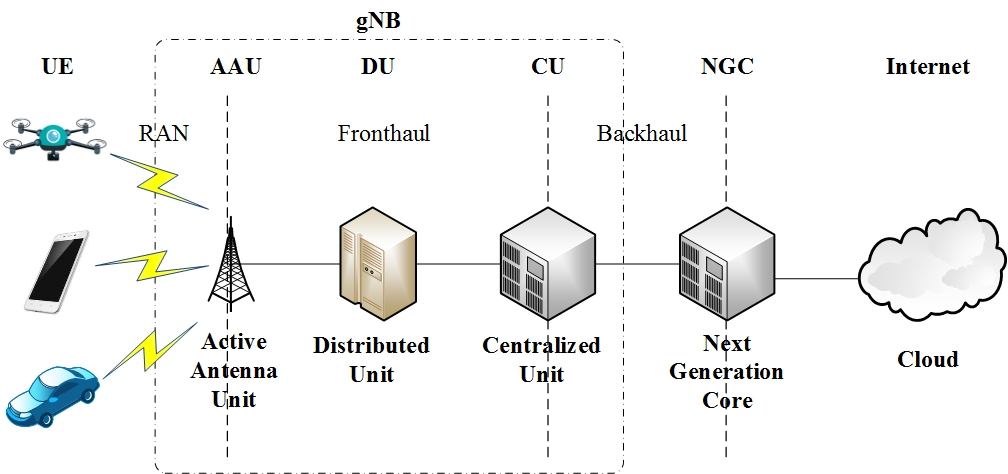
\includegraphics[width=\textwidth]{5G_delay_en.jpg}
\caption{5G network architecture.}
\label{fig_architecture}
\end{figure*}

\subsection{Delay of URLLC Network}
UE devices firstly access to AAU. The AAU is actually a part of base station. This part of the communication belongs to RAN.
UE's data will be accepted by AAU, and AAU put forward the data to DU.
There are two situations when data arrive at DU.
If CU and DU are deployed together, the data can be arrived at CU immediately. Otherwise, the data will be sent to CU from DU.
The communication from AAU to CU belongs to fronthaul.
The data leave CU and continue upward to the NGC. This part of the communication is called hackhaul.
NGC will process the data and it will take some time.
Finally, NGC sends the data to Cloud servers. The unidirectional transmission is finished.

So the whole delay or latency in 5G system is contribute by the time processing of RAN, fronthual, backhaul, Core Network and Cloud server. It can be expressed as (\ref{eq_urllc_delay_composition}).
\begin{equation}\label{eq_urllc_delay_composition}
T_{Total} = T_{RAN} + T_{Fronthaul} + T_{Backhaul} + T_{NGC} + T_{Cloud}
\end{equation}
where
\begin{itemize}
\item $T_{RAN}$ is the time cost by physical layer transmission between UEs and AAU.
\item $T_{Fronthaul}$ is the delay between AAU to CU. It is the time taken in gNB.
\item $T_{Backhaul}$ is the time taken to communication between gNB to NGC.
\item $T_{NGC}$ is the delay taken place in NGC.
\item $T_{Cloud}$ is the latency which data transmission between NGC and Cloud server.
\end{itemize}
To meet the URLLC key requirement, we should do a good job of studying $T_{Total}$.
In this part, we discuss the latency mainly on the User Plane (UP) rather than Control Plane (C-Plane).
That because most of latency is attributed to the UP.
UP latency is the communication time between UE and network nodes when transmission and reception of the data at the corresponding IP layer.
Whereas, the C-Plane latency is the time spend on radio resource allocating and state switching from idle to active.
Compared with UP latency, the C-Plane delay is tiny and can be ignored.
\subsection{Problem Description}
The data is transferred from UE, through each nodes, and finally to the cloud.
According to the requirement of URLLC, the reliability and random latency \cite{article_MF_Random} can be described as (\ref{eq_urllc_delay_problem}):

\begin{equation}\label{eq_urllc_delay_problem}
P\{delay > d \} < \epsilon
\end{equation}

The delay should be within 1ms, so the $d < 1$, the unit is millisecond (ms).
Where $\epsilon$ is defined as a very small probability.
%Meanwhile the block error rate (BLER) must be 99.999\%.
%It means that the value of $\epsilon$ must be less than $1*10^{-5}$, (i.e. $1 - 1*10^{-5} = 0.99999$, It equals to BLER $99.999\%$).
The Formula.\ref{eq_urllc_delay_problem} represents the 5G URLLC network successfully transport data and satisfy the delay requirements.
%and reliability

\subsection{Stochastic Network Calculus}
In SNC theory, the min-plus algebra is applied to analyze queuing system.
Let $\mathcal{F}$ denotes the set of non-negative non-decreasing functions and $\mathcal{\bar{F}}$ denotes the set of non-negative non-increasing function.
We employ the cumulative process to represent amount of traffic flow.
Arrival process, departure process and service process are denoted as $A(t)$, $D(t)$, and $S(t)$ respectively.
For any $0 \leq s \leq t, A(0)=0, A(s,t) = A(t) - A(s)$, and practical significance of $A(t)$ is the cumulative arrival data at time $t$.
It same to the $D(t)$ and $S(t)$.
Some fundamental definitions of curve are well described in literature \cite{book1}.
We utilize and expand the following in this paper.

\begin{definition}\label{def_SAC}
{\bfseries (Stochastic Arrival Curve)}.
A flow is said to have a stochastic arrival curve $\alpha\in\mathcal{F}$ with bounding function $f\in\mathcal{\bar{F}}$, denoted by $A(t) \sim <f,\alpha>$, if for all $t \geq 0$ and all $x\geq0$ there holds
\begin{equation}\label{eq_sac}
P\Bigl\{\sup_{0\leq s \leq t}\{A(s,t) - \alpha(t-s)\} > x \Bigr\} \leq f(x).
\end{equation}
\end{definition}
Where $\alpha(\tau)$ is the stochastic arrival curve, and it denotes the maximum of flow $A(\tau)$.
Function $f(x)$ denotes the violation probability.
It assumes that the stochastic arrival curve $\alpha(\tau)$ may be exceeded by arrival process $A(\tau)$ in sometimes, but the probability of being exceeded is constrained by the boundary function $f(x)$.

\begin{definition}\label{def_SSC}
{\bfseries(Stochastic Service Curve)}. A system $S$ is said to provide a stochastic service curve $\beta\in\mathcal{F}$ with bounding function $g \in \mathcal{\bar{F}}$, denoted by $S \sim<g, \beta>$, if for all $t\geq0$ there holds
\begin{equation}\label{eq_ssc}
P\Bigl\{\sup_{0\leq s \leq t}[A\otimes\beta(s) - D(s)] > x \Bigr\} \leq g(x).
\end{equation}
\end{definition}
%Current editing!

The symbol $\otimes$ represents the cumulative min-plus convolution operation.
Which
\begin{equation}\label{eq_convolution}
A\otimes\beta(t) = \inf_{0 \leq s \leq t}\{A(s)+\beta(s,t)\}
\end{equation}
$\beta(t)$ is the stochastic service curve which means the worst service capability provided by the server.
Similar to the stochastic arrival curve, the data that already have been served are probably to be more than the data left.
The probability of producing exceeding data can be constrained by the boundary function $g(x)$.

Similarly as in (\ref{eq_ssc}), the departure process relates to the arrival and service process and it is described as
\begin{equation}\label{eq_departure}
D(t) \geq \inf_{0\leq s \leq t}\{A(s)+ S(s,t)\} =  A \otimes S(t).
\end{equation}
Where for all $s,t \geq 0$ and $s \leq t$.
That is also the concept of a dynamic server which mentioned in \cite{article1}.
From the (\ref{eq_departure}), we can better understand the relationship among arrival process, departure process and service process.
With these basic processes and curves, we can discuss the definition of the delay boundary.

\begin{definition}\label{def_delay_process}
{\bfseries(Latency Process)}.
Let $A(t)$ and $D(t)$ respectively be the arrival process and departure process.
The latency process $L(t)$ at time $t \geq 0$ is defined as
\begin{equation}\label{eq_delay_define}
L(t) = \inf\{d \geq 0 : A(t) \leq D(t+d)\}.
\end{equation}
\end{definition}

The (\ref{eq_delay_define}) express that latency $L(t)$ is the least value of $d$, and the $d$ must meet the condition which the amount of arrival data at time $t$ is less than or equal to the departure data at time $t+d$.
It also means that the data do not leave the server immediately.
The duration of the data in server is the delay time.
In Formula.\ref{eq_delay_define}, the arrival process $A(t)$ is little than or equal to the departure process $D(t+d)$.
It means that the data arrived in server at time $t$ are all leaving from server at time $t+d$.
If $A(t)$ is large than or equal to the departure process $D(t+d)$, that represents the data arrived at $t$ moment have not been completed by service during $d$ period of time.
So the $A(t)$ little than or equal to $D(t+d)$ situation is utilized to describe the shortest time that server takes for the data to be serviced.
That is the latency or delay.

According to the latency process definition, and utilizing stochastic arrival process and stochastic service process, so the stochastic latency bound has been defined at following.
%we have the result for stochastic latency bound.

\begin{theorem}\label{thrm_latency}{\bfseries (Stochastic Latency Bound)}
A system with an input process $A(t)$.
$A(t)$ is a stochastic arrival process with stochastic arrival curve $\alpha \in \mathcal{F}$ and bounded by function $f \in \mathcal{\bar{F}}$ (i.e., $A \sim <f, \alpha>$).
The system provides to the input a stochastic service process $S(t)$.
$S(t)$ is with stochastic service curve $\beta \in \mathcal{F}$ with bounding function $g \in \mathcal{\bar{F}}$ (i.e., $S \sim <g, \beta>$).
Then, for all $t\geq 0$ and $x \geq 0$, the Latency $L(t)$ is bounded by
\begin{equation}
P\{L(t)>h(\alpha+x, \beta)\}\leq f \otimes g(x)
\end{equation}
\end{theorem}
Where function $h(\alpha+x, \beta)$ denotes the maximum horizontal distance between $\alpha+x$ and $\beta$, the express $f \otimes g(x)$ represents the cumulative min-plus convolution operation of function $f$ and $g$.

\begin{theorem}\label{thrm_concatenation}{\bfseries (Concatenation Property)}
Considering a flow passes through a network of $N$ server nodes in tandem.
If each server nodes $n(=1,2,...,N)$ provides a stochastic service curve $S^{n}\sim<g^{n}, \beta^{n}>$ to its input, then the network guarantees to the flow a stochastic service curve $S\sim<g,\beta>$ with
\begin{equation}
\begin{split}
\beta(t)=\beta^{1}\otimes\beta^{2}\otimes\cdot\cdot\cdot\otimes\beta^{N}(t) \\
g(x)=g^{1}\otimes g^{2}\otimes\cdot\cdot\cdot\otimes g^{N}(t)
\end{split}
\end{equation}
\end{theorem}

\subsection{Model Building}
The network character of URLLC can be described as a dynamic server by stochastic processes as introducing in above.
The data sent by UE can be represented by the arrival process $A(t)$.
The service capacity provided by the network server node can be depicted as the stochastic service process $S(t)$.

As assumption the latency of URLLC in Formula.\ref{eq_urllc_delay_composition}, we consider the URLLC network is a tandem system.
So the delay of URLLC should fall in the concatenation characterization in SNC.

We consider that a UE's network flow passing through the gNB, CN and Cloud in tandem mode.
Each network node $k(=gNB, AAU, DU, CU, CN, Cloud)$ provides a stochastic service curve $S_{k}\sim<g_k, \beta_k>$ to its flow.
We first discuss about the gNB subsystem.
The gNB includes AAU, DU and CU, so $S_{AAU}(s,t)$, $S_{DU}(s,t)$ and $S_{CU}(s,t)$ are in series.
We use the same indices to denote the arrival and departure process of the respective systems.
Especially the source of data is from UE.
So $A_{AAU}(t)$ as arrival process denotes the input data of AAU from UE in gNB subsystem.
The arrival process of DU $A_{DU}(t)$ actually equals to the departure process of AAU $D_{AAU}(t)$, where $A_{DU}(t) = D_{AAU}(t)$.
By the same token, $A_{CU}(t) = D_{DU}(t)$ similarly for CU server.
The departure process of CU is $D_{CU}(t)$.
It is also the departure process of the gNB subsystem.

Consider the gNB subsystem is tandem deploy, we assume that the AAU server provides a $S_{AAU}(t)$ capacity to deal with the arrival data.
Applying (\ref{eq_departure}), the departure process can be represent as
\begin{equation} \label{eq_departure_AAU}
D_{AAU}(t)\geq A_{AAU}\otimes S_{AAU}(t).
\end{equation}
Similar to the departure process of AAU, we can get the process of DU
\begin{equation}\label{eq_departure_DU}
D_{DU}(t) \geq A_{DU}\otimes S_{DU}(t).
\end{equation}
Because of $A_{DU}(t) = D_{AAU}(t) = A_{AAU}\otimes S_{AAU}(t)$, we put (\ref{eq_departure_AAU}) into (\ref{eq_departure_DU}) to replace $A_{DU}(t)$ by $A_{AAU}\otimes S_{AAU}(t)$ and get
\begin{equation}\label{eq_departure_DU2}
D_{DU}(t) \geq (A_{AAU}\otimes S_{AAU}(t))\otimes S_{DU}(t).
\end{equation}
By recursive insertion, we can obtain
\begin{equation}\label{eq_departure_CU}
D_{CU}(t) \geq ((A_{AAU}\otimes S_{AAU}) \otimes S_{DU})\otimes S_{CU}(t).
\end{equation}
Applying the associativity of min-plus convolution, it holds that
\begin{equation}
\begin{split}
D_{CU}(t) &\geq ((A_{AAU}\otimes S_{AAU}) \otimes S_{DU})\otimes S_{CU}(t) \\
&\geq A_{AAU}\otimes (S_{AAU}\otimes S_{DU} \otimes S_{CU})(t).
\end{split}
\end{equation}
From the gNB subsystem perspective to see, $A_{AAU}(t)$ is the first input and $D_{CU}(t)$ is the last output of gNB.
So $A_{AAU}(t)$ equal to $A_{gNB}(t)$, and $D_{CU}(t)$ is the departure process of the gNB $D_{gNB}(t)$.
Then we can get gNB subsystem
\begin{equation}\label{eq_departure_gNB}
D_{gNB} \geq A_{AAU}\otimes (S_{AAU}\otimes S_{DU} \otimes S_{CU})(t).
\end{equation}
Assuming first-come first-served order, we use Definition.\ref{def_delay_process} and equation (\ref{eq_departure_gNB}), and let $L_{gNB}$ denotes the latency process of gNB, there holds
\begin{equation}\label{eq_latency_gNB}
\begin{split}
L_{gNB}(t) &= \inf\{d\geqslant0: A_{gNB}(t) - D_{gNB}(t+d) \leqslant 0 \} \\
 &= \inf\{d\geqslant0: A_{AAU}(t) - D_{CU}(t+d) \leqslant 0 \}  \\
 &= \inf\{d\geqslant0: A_{AAU}(t) \\
 &  - A_{AAU}\otimes (S_{AAU}\otimes S_{DU} \otimes S_{CU})(t+d) \leqslant 0 \}
\end{split}
\end{equation}

With Theorem.\ref{thrm_latency} and Theorem.\ref{thrm_concatenation}, the delay bound can be analysis by following corollary.

\begin{corollary}\label{crl_latency}{\bfseries (Latency Bound of gNB)}
In gNB subsystem, $A_{AAU}(t)$ is a stochastic arrival process with stochastic arrival curve $\alpha_{AAU}$, i.e. $A \sim <f_{AAU}, \alpha_{AAU}>$.
 $\alpha_{AAU} \in \mathcal{F}$, $f_{AAU} \in \mathcal{\bar{F}}$.
The server nodes in subsystem provide stochastic service process $S_{AAU}(t), S_{DU}(t), S_{CU}(t)$ respectively, i.e.
$S_{AAU} \sim <g_{AAU},\beta_{AAU}>, S_{DU}\sim <g_{DU},\beta_{DU}>, S_{CU}\sim <g_{CU}, \beta_{CU}>$.
And $\beta_{AAU},\beta_{DU},\beta_{CU} \in \mathcal{F}$, $g_{AAU}, g_{DU}, g_{CU} \in \mathcal{\bar{F}}$.
Then, for all $t\geq 0$ and $x \geq 0$, the Latency of gNB subsystem $L_{gNB}(t)$ is bounded by
\begin{equation}
\begin{split}
P\{L_{gNB}(t) \geq d\} &= P\{L_{gNB}(t) \geq h(\alpha_{AUU}+x, \beta_{gNB})\} \\
 &\leqslant f_{AAU}\otimes g_{gNB}(x)
\end{split}
\end{equation}
\end{corollary}
where service rate $\beta_{gNB}(t)=\beta_{AAU}\otimes \beta_{DU}\otimes \beta_{CU}(t)$, and bound function $g_{gNB}=g_{AAU}\otimes g_{DU}\otimes g_{CU}(x)$.

$Proof:$ Please see Appendix A.

For mobile edge computing (MEC) deployment, CU can be the end of the transmission. That because the computing resource and storage resource are located at CU.
The Corollary.\ref{crl_latency} is suitable for analysis the delay of communication from UE to CU.
However, in order to comprehensively discuss the delay of URLLC system, we need to convert the destination from CU to Cloud.
By extending Corollary.\ref{crl_latency}, we can draw the whole URLLC system latency bound.
\begin{corollary}\label{crl_latency_urllc}{\bfseries (Latency Bound of URLLC)}
In 5G URLLC system, $A_{AAU}(t)$ is a stochastic arrival process with stochastic arrival curve $\alpha_{AAU}$, i.e. $A\sim<f_{AAU},\alpha_{gNB}>$. $\alpha_{AAU}\in\mathcal{F}$, $f_{AAU}\in\mathcal{\bar{F}}$.
The server nodes in URLLC system provide stochastic service process $S_{gNB}(t)$, $S_{NGC}(t)$ and $S_{Cloud}(t)$ respectively, i.e.
$S_{gNB}\sim<g_{gNB},\beta_{gNB}>$, $S_{NGC}\sim<g_{NGC},\beta_{NGC}>$, and $S_{Cloud}\sim<g_{Cloud},\beta_{Cloud}>$.
Service rate $\beta_{gNB},\beta_{NGC},\beta_{Cloud}\in\mathcal{F}$, $g_{gNB}, g_{NGC}, g_{Cloud}\in\mathcal{\bar{F}}$.
Then, for all $t\geq 0$ and $x \geq 0$, the Latency of URLLC system $L_{All}(t)$ is bounded by
\begin{equation}\label{eq_in_crl_2}
\begin{split}
P\{L_{All}(t) \geq d\} &= P\{L_{All}(t) \geq h(\alpha_{AUU}+x, \beta_{All})\} \\
 &\leqslant f_{AAU}\otimes g_{All}(x)
\end{split}
\end{equation}
\end{corollary}
where $\beta_{All}(t)=\beta_{gNB}\otimes \beta_{NGC}\otimes \beta_{Cloud}(t)$, and $g_{All}=g_{gNB}\otimes g_{NGC}\otimes g_{Cloud}(x)$.

$Proof:$ Please see Appendix B.
We have built a model to represent the latency of 5G MEC (UE to gNB) and URLLC (the full path from UE to Cloud).
Next we intend to calculate the delay boundary of the model.
With Corollary.\ref{crl_latency_urllc}, we know that 4 key variance need to be determined. These are stochastic arrival process $\alpha_{AAU}$, $f_{AAU}$, and stochastic service process $\beta_{All}$, $g_{All}$.
Especially, we can also decompose $\beta_{All}$ and $g_{All}$ to obtain more detailed result.

In URLLC scenario, the data is usually fixed unit packet size, the data size sometimes very tiny while applying millimeter-wave technology.
We assume that UE data arrive will approximate to a Poisson distribution with mean rate $\lambda$.
So arrive curve $\alpha_{AAU}=\lambda t$ and bound function will be
\begin{equation}\label{eq_f_1}
f_{AAU}(x)=\sum_{k=x+\lambda t}^{\infty} \frac{e^{\lambda t}\cdot (\lambda t)^{k}}{k!}
\end{equation}
With MGF of right hand in (\ref{eq_f_1}) and Chernoff bound, $f_{AAU}$ can be tighten by
\begin{equation}\label{eq_f_2}
f_{AAU}(x)=e^{x-(\lambda t+x)ln\frac{\lambda t+x}{\lambda t}}
\end{equation}
The proof of this part can be found in \cite{proc_jiang_On}.
Two variances in stochastic arrival process have been solved.
We begin to determine $\beta_{All}$, $g_{All}$ for the stochastic service process.

In order to simplify the problem, we generalize service rate of server nodes and assume that each node provides data processing capacity as $\beta(t)=Ct$ with bounding function $g(x)=ae^{-bx}$.
According to Corollary.\ref{crl_latency_urllc}, we can get
\begin{equation}
g_{All}(x)=g_{AAU}\otimes g_{DU}\otimes g_{CU}\otimes g_{NGC}\otimes g_{Cloud}(x)
\end{equation}
Therefore,
\begin{equation}
\begin{split}
g_{All}(x)&=g_{AAU}\otimes g_{DU}\otimes g_{CU}\otimes g_{NGC}\otimes g_{Cloud}(x)  \\
&=\inf_{x_{1}+x_{2}+x_{3}+x_{4}+x_{5}=x}\sum_{k=1}^{5}a_{k}e^{-b_{k}x_{k}}
\end{split}
\end{equation}
Applying with the conclusion in \cite{proc_jiang_Wireless}, we can hold
\begin{equation}
\begin{split}
&\inf_{x_{1}+x_{2}+x_{3}+x_{4}+x_{5}=x}\sum_{k=1}^{5}a_{k}e^{-b_{k}x_{k}} = e^{\frac{-x}{w}}\prod_{k=1}^{5}(a_{k}b_{k}w)^{\frac{1}{b_{k}w}}
\end{split}
\end{equation}
where $w=\sum_{k=1}^{5}\frac{1}{b_{k}}$, and service bound functions respectively are $g_{AAU}(x)=a_{1}e^{-b_{1}x_{1}}$, $g_{DU}(x)=a_{2}e^{-b_{2}x_{2}}$, $g_{CU}(x)=a_{3}e^{-b_{3}x_{3}}$, $g_{NGC}(x)=a_{4}e^{-b_{4}x_{4}}$, $g_{Cloud}(x)=a_{5}e^{-b_{5}x_{5}}$.
with all the information we discuss above,  and applying the lemma which proved in \cite{proc_jiang_Wireless}, we can get
\begin{equation}\label{eq_g_all}
g_{All}(x) = e^{\frac{-xb}{n+1}}(a(n+1))
\end{equation}
We put (\ref{eq_f_2}), (\ref{eq_g_all}) into (\ref{eq_in_crl_2}) and apply the Theorem.3 proved in \cite{proc_Michael}, it can be derived that
\begin{equation}\label{eq_latency_f_g}
\begin{split}
&P\{L(t)>h(\alpha_{AAU}+x, \beta)\} \\
&= P\{L(t)>\frac{x}{C-\lambda}\} \\
&\leq e^{x-(\lambda t+x)ln\frac{\lambda t+x}{\lambda t}}\cdot e^{\frac{-xb}{n+1}}(a(n+1))
\end{split}
\end{equation}
Then we hold the latency bound as (\ref{eq_urllc_delay_problem}).
Let $d=\frac{x}{C-\lambda}$ and set the right side of (\ref{eq_latency_f_g}) equal to $\epsilon$. The $\epsilon$ is a small latency bound violation probability. We can obtain a relationship between $d$ and $\epsilon$.
\begin{equation}
d = \frac{1}{C-\lambda}\cdot\frac{n+1}{b}\cdot ln{\frac{a(n+1)}{\epsilon}}
\end{equation}
The calculation process can be found in Appendix C.

\section{Numerical Results and Performance Evaluation}
%In this section, we will validate the analysis result and discuss what factors are the main cause of latency in URLLC.
In this section, we will discuss what factors are the main cause of latency in URLLC.

Although the deployment details of the URLLC standard are not yet released, we can still apply SNC theory for quantitative analysis.
We assume that the 5G URLLC networks are standalone deployment.
The packet arrival rate is constant and arrival process satisfies Poisson distribution.
A general URLLC reliability requirement for one transmission of a packet is $1*10^{-5}$ for 32 bytes with a user plane latency of 1ms.
So we set the violation probability value around $1*10^{-5}$.
More simulation parameters can be found in Table.\ref{tab_2}.

\begin{table}
  \caption{evaluation parameters}\label{tab_2}
  \center
  \begin{tabular}{|l|l|}
    \hline
    Parameter & Value \\
    \hline
    Network deployment & Standalone   \\
    Traffic mode & Constant transmission, Poisson arrival \\
    Arrival rate $\lambda$ & 20 (Gbit/s)    \\
    Service rate C & 40,45,50,55 (Gbit/s)    \\
    Service bound a & 1 \\
    Service bound b & 3 \\
    Number of tandem servers n & 5    \\
    Violation probability & $1*10^{-5}$ \\
    Latency bound & 1 (ms)  \\
    \hline
  \end{tabular}
  \center
\end{table}
Taking this boundary probability as the precondition, we simulate the relationship between system latency and service rate by applying the conclusions we have drawn in the previous section.
Fig.\ref{fig2} provide the evaluated URLLC delay with different service rate under violation probability $1*10^{-5}$.
The value of violation probability is from $5*10^{-6}$ to $15*10^{-6}$.
We arrange the value scope to include the demand value $1*10^{-5}$ to observe the effect of this value on delay.
We adopt 4 service rates in model and all the curves are slow down by violation probability value. From this we can conduct that the violation probability is not the main factor to influence the latency.
\begin{figure}[htbp]
  \centering
  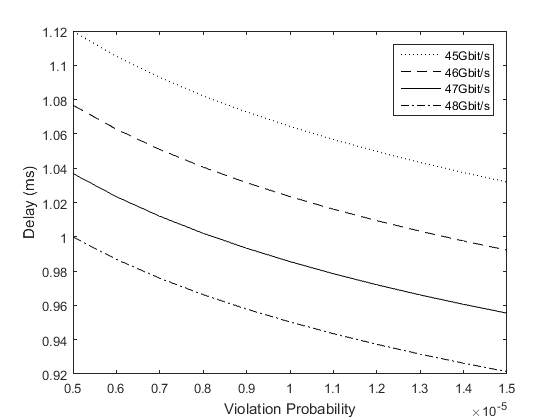
\includegraphics[width=.5\textwidth]{delay_no_tandem.png}
  \caption{Service Rate Influence}
  \label{fig2}
\end{figure}
In order to make the delay less than 1ms, we set service rate from 45Gbit/s to 48Gbit/s based on arrival rate 20Gbit/s.
We can procure that delay approximates 1ms when service rate is 47Gbit/s at violation probability $1*10^{-5}$.
As the service rate increases, the delay of the system will decrease.
When service rate is 48Gbit/s, system latency can approach 1ms with lower violation probability.
That means system can guarantee the low latency communication in a stable state.

Fig.\ref{fig3} presents the relationship among latency, number of server levels and service rate.
The arrival rate is constant and speed is 20Gbit/s. The violation probability is maintained at $1*10^{-5}$.
Based on the above setting, we can derived that the delay is sensitive on number of server levels.
From Fig.\ref{fig3}, we can see the slope of latency cause by number of server levels in tandem is larger than the service rate.
We draw a delay equals 1ms flat plane to cut the curve surface.
The part below the plane is the scope of deployment parameters which satisfying the delay condition.
In order to ensure low latency of communication, it is necessary to reduce the levels of system deployment as much as possible and increase the service rate of each server layer.

\begin{figure}[htbp]
  \centering
  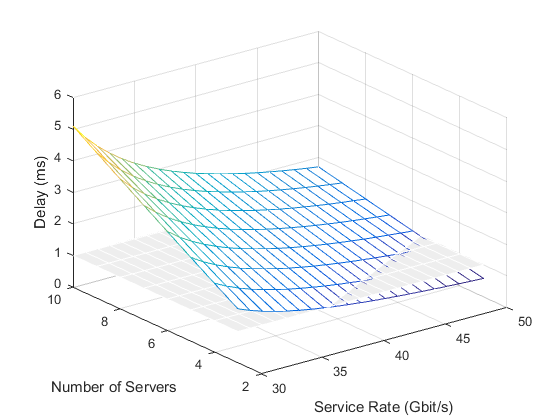
\includegraphics[width=.5\textwidth]{delay_servers.png}
  \caption{Number of Server Levels Influence}
  \label{fig3}
\end{figure}

\section{Conclusions}
In this paper, the architecture of 5G URLLC network researched.
According to the architecture characteristics, the URLLC network is modeled as a tandem system which demonstrate the communication from UE to Cloud.
Applying stochastic network theory and combining the features of URLLC network, performance analysis has been conducted.
We have investigated the relationship among: the delay constraint, the service rate, violation probability and the number of deployment servers levels in URLLC networks.
The 3GPP standard is taken into account when we set the simulation parameters.
Numerical results are demonstrate that the main factor which can impact on latency is number of server deployment levels.
That also means Edge Computing will be the trend in URLLC application deployment.
The service rate of the server is also a factor affecting the delay. With the increase of service rate, delay can be reduced.
The results derived from evaluation which provide valuable guidelines for the early design of URLLC deployment.
With the further development of the researches, we would consider to include handover access in URLLC communication.

\section{Appendix}
\subsection{Proof of Corollary.1}
\begin{proof}
Since the latency process Definition.(\ref{def_delay_process}) are defined as $L(t) = \inf\{d \geq 0 : A(t) \leq D(t+d)\}$,
event ${L(t)} > d$ implies event ${A(t)\leq D(t+d)}$.
We move $D(t+d)$ from right hand to left hand, and according to (\ref{eq_latency_gNB}), the latency bound of gNB can be hold as
\begin{equation}\label{eq_latencybound_gNB}
P\{L_{gNB}(t)>d\} \leqslant P\{A_{AAU}(t) - D_{CU}(t+d) \leq 0\}
\end{equation}

Then we focus on the $\{A_{AAU}(t) - D_{CU}(t+d)\}$ part. We put right hand of (\ref{eq_departure_gNB}) into this part, we can get
\begin{equation}\label{zm_1}
\begin{split}
 &A_{AAU}(t) - D_{CU}(t+d) \\
=&A_{AAU}(t) - A_{AAU}\otimes (S_{AAU}\otimes S_{DU}\otimes S_{CU})(t+d)\\
+&A_{AAU}\otimes (S_{AAU}\otimes S_{DU}\otimes S_{CU})(t+d)-D_{CU}(t+d)\\
\end{split}
\end{equation}

With the Theorem.\ref{thrm_concatenation}, utilizing the concatenation property we can obtain that
$S_{AAU}\sim<g_{AAU},\beta_{AAU}>$, $S_{DU}\sim<g_{DU},\beta_{DU}>$, $S_{CU}\sim<g_{CU},\beta_{CU}>$.
Stochastic service process convolution operation $(S_{AAU}\otimes S_{DU}\otimes S_{CU})$ means gNB subsystem provides maybe lower than $(\beta_{AAU}\otimes \beta_{DU} \otimes \beta_{CU})$ processing capacity,
but the violation probability in this case is limited by $g_{AAU}\otimes g_{DU}\otimes g_{DU}$.
Through applying (\ref{eq_ssc}), we denote $\beta_{gNB}$ equals to $(\beta_{AAU}\otimes \beta_{DU} \otimes \beta_{CU})$,
$g_{gNB}$ equals to $g_{AAU}\otimes g_{DU}\otimes g_{DU}$.
hence (\ref{zm_1}) can hold be
\begin{equation}\label{zm_2}
\begin{split}
 &A_{AAU}(t) - D_{CU}(t+d) \\
=&A_{AAU}(t) - A_{AAU}\otimes (\beta_{AAU}\otimes \beta_{DU}\otimes \beta_{CU})(t+d)\\
 &+A_{AAU}\otimes (\beta_{AAU}\otimes \beta_{DU}\otimes \beta_{CU})(t+d) - D_{CU}(t+d) \\
=&A_{AAU}(t) - A_{AAU}\otimes \beta_{gNB}(t+d) \\
 &+A_{AAU}\otimes \beta_{gNB}(t+d) - D_{CU}(t+d)
\end{split}
\end{equation}
According to (\ref{eq_convolution}), we replace $A_{AAU}\otimes \beta_{gNB}(t+d)$ by $\inf\{A_{AAU}(s)+\beta_{gNB}(t+d-s)\}$ in (\ref{zm_2}).
Consequently,
\begin{equation}\label{zm_3}
\begin{split}
 &A_{AAU}(t) - D_{CU}(t+d) \\
=&A_{AAU}(t) - A_{AAU}\otimes \beta_{gNB}(t+d) \\
 &+A_{AAU}\otimes \beta_{gNB}(t+d) - D_{CU}(t+d) \\
=&A_{AAU}(t) - \inf_{0\leqslant s \leqslant t+d}\{A_{AAU}(s)+ \beta_{gNB}(t+d-s)\} \\
 &+A_{AAU}\otimes \beta_{gNB}(t+d) - D_{CU}(t+d)\\
\leq&A_{AAU}(t) - A_{AAU}(s) - \beta_{gNB}(t+d-s)\} \\
 &+A_{AAU}\otimes \beta_{gNB}(t+d) - D_{CU}(t+d)  \\
\leq&A_{AAU}(s,t) - \alpha_{AAU}(t-s)\\
 &+\alpha_{AAU}(s,t)-\beta_{gNB}(t+d-s)\\
 &+A_{AAU}\otimes \beta_{gNB}(t+d) - D_{CU}(t+d)  \\
\end{split}
\end{equation}

We add $\alpha_{AAU}$ at step 4 in (\ref{zm_3}) to build stochastic arrival curve.
Based on the stochastic arrival curve (\ref{eq_sac}),$A_{AAU}(s,t) - \alpha_{AAU}(s,t)$ is less than or equal to $f_{AAU}$.
Applying stochastic service curve (\ref{eq_ssc}), $A_{AAU}\otimes \beta_{gNB}(t+d) - D_{CU}(t+d)$ is less than or equal to $g_{gNB}$.
With Theorum.\ref{thrm_latency}, we use $h(\alpha+x, \beta)$ replace the $d$. where $h(\alpha+x,\beta)$ is the maximum horizontal distance between $\alpha+x$ and $\beta$ for $x \geq 0$. The $h(\alpha,\beta)$ function implies the condition
\begin{equation}\label{condition}
\lim_{t\rightarrow\infty}[\alpha(t)-\beta(t)]\leq 0.
\end{equation}
we can obtain
\begin{align*}
&P\{L(t)>h(\alpha_{AAU}+x, \beta_{gNB})\} \\
&= P\{\{A_{AAU}(t) - D_{CU}(t+h(\alpha+x, \beta))\} > 0\}  \\
&\leqslant \sup_{0\leqslant s \leqslant t}\{A_{AAU}(s,t)-\alpha_{AAU}(t-s)\}  \\
&+\sup_{0\leqslant s \leqslant t+h(\alpha_{AAU}+x, \beta_{gNB})}\{A_{AAU}\otimes \beta_{gNB}(s)-D_{CU}(s)\} \\
&\leqslant f_{AAU}(t)+g_{gNB}(x) \\
&\leqslant \inf\{f_{AAU}(t)+g_{gNB}(x-t)\} \\
&\leqslant f_{AAU}\otimes g_{gNB}(x)
\end{align*}
Therefore, Corollary.\ref{crl_latency} is proved.
\end{proof}

\subsection{Proof of Corollary.2}
\begin{proof}
In the Corollary.\ref{crl_latency}, the gNB subsystem are constituted by AAU, DU and CU. In addition to gNB, the whole 5G URLLC system also include NGC and Cloud.
%ֻ��Ҫ���������һЩ�ʵ��Ļ����Ϳ����ˡ�
According to the concatenation property which mentioned in Theorem.\ref{thrm_concatenation}, then the network guarantees to the flow a stochastic service curve $S_{All}\sim<g_{All},\beta_{All}>$ with
\begin{equation}\label{eq_tandem_beta_top}
\beta_{All}(t)=\beta_{gNB}\otimes\beta_{CN}\otimes\beta_{Cloud}(t)
\end{equation}
where
\begin{equation}\label{eq_tandem_beta_gNB}
\beta_{gNB}(t)=\beta_{AAU}\otimes\beta_{DU}\otimes\beta_{CU}(t)
\end{equation}
actually
\begin{equation}\label{eq_tandem_beta_all}
\beta_{All}(t)=\beta_{AAU}\otimes\beta_{DU}\otimes\beta_{CU}\otimes\beta_{CN}\otimes\beta_{Cloud}(t)
\end{equation}
and
\begin{equation}\label{eq_tandem_g_top}
g_{All}(x)=g_{gNB}\otimes g_{CN}\otimes g_{Cloud}(x)
\end{equation}
where
\begin{equation}\label{eq_tandem_g_gNB}
g_{gNB}(x)=g_{AAU}\otimes g_{DU}\otimes g_{CU}(x)
\end{equation}
actually
\begin{equation}\label{eq_tandem_g_all}
g_{All}(x)=g_{AAU}\otimes g_{DU}\otimes g_{CU}\otimes g_{CN}\otimes g_{Cloud}(x)
\end{equation}
Based on latency process Definition.(3), the 5G URLLC system latency process can be defined as
\begin{equation}
L(t) = \inf\{d \geqslant 0: A_{AAU}(t) \leq D_{Cloud}(t+d)\}
\end{equation}
Latency bound of 5G URLLC is defined as
\begin{equation}
P\{L(t)\geq d\} = P\{A_{AAU}(t)-D_{Cloud}(t+d)\leq 0\}
\end{equation}
We also focus on $A_{AAU}(t)-D_{Cloud}(t+d)$ part.
where $D_{Cloud}\geqslant A_{AAU}\otimes S_{AAU}\otimes S_{DU}\otimes S_{CU}\otimes S_{NGC}\otimes S_{Cloud}$. Then we have
\begin{align*}
&A_{AAU}(t)-D_{Cloud}(t+d)\\
=&A_{AAU}(t)-A_{AAU}\otimes S_{AAU}\otimes S_{DU}\otimes S_{CU}\\
&\otimes S_{NGC}\otimes S_{Cloud}(t+d)\\
&+A_{AAU}\otimes S_{AAU}\otimes S_{DU}\otimes S_{CU}\\
&\otimes S_{NGC}\otimes S_{Cloud} -D_{Cloud}(t+d)\\
=&A_{AAU}(t)-A_{AAU}\otimes S_{gNB}\otimes S_{NGC}\otimes S_{Cloud}(t+d)\\
&+A_{AAU}\otimes S_{gNB}\otimes S_{NGC}\otimes S_{Cloud} -D_{Cloud}(t+d)\\
\leq&A_{AAU}(t)-A_{AAU}(s)\\
&-\beta_{gNB}\otimes\beta_{NGC}\otimes\beta_{Cloud}(t+d-s))\\
&+A_{AAU}\otimes S_{gNB}\otimes S_{NGC}\otimes S_{Cloud} -D_{Cloud}(t+d)\\
\leq&A_{AAU}(s,t)-\alpha_{AAU}(t-s)\\
&+\alpha_{AAU}(t-s)-\beta_{all}(t+d-s)\\
&+A_{AAU}\otimes \beta_{all}(t+d)-D_{Cloud}(t+d)
\end{align*}
With stochastic arrival curve (\ref{eq_sac}), $A_{AAU}(s,t)-\alpha(t-s)$ is bounded by $f_{AAU}(x)$.
According to stochastic service curve (\ref{eq_ssc}), $A_{AAU}\otimes \beta_{All}(t+d)-D_{Cloud}(t+d)$ is limited by $g_{All}$.
For long-term running, if $t\rightarrow\infty$, $\alpha_{AAU}(t-s)-\beta_{All}(t+d-s)$ approximate to zero because of $\alpha_{AAU},\beta_{All}\in\mathcal{F}$.
Finally, with Theorem.\ref{thrm_latency}, the delay of the URLLC system can be bounded by this
\begin{equation}\label{eq_latency_urllc}
P\{L(x)>h(\alpha_{AAU}+x, \beta_{All})\} < f_{AUU} \otimes g_{All}(x)
\end{equation}
Therefore, Corollary.2 is proved.
\end{proof}

\subsection{Calculation of Delay}
We first set right side of (\ref{eq_latency_f_g}) equals to $\epsilon$, and we logarithm on both sides then hold
\begin{equation}\label{eq_appendixC_1}
\begin{split}
&e^{x-(\lambda t+x)ln\frac{\lambda t+x}{\lambda t}}\cdot e^{\frac{-xb}{n+1}}(a(n+1)) = \epsilon \\
&e^{x-(\lambda t+x)ln\frac{\lambda t+x}{\lambda t}}\cdot e^{\frac{-xb}{n+1}} = \frac{\epsilon}{a(n+1)}
\end{split}
\end{equation}
for a long-term running situation, $t\rightarrow\infty$, then
\begin{equation}
\lim_{t\rightarrow\infty}(\lambda t+x)ln\frac{\lambda t+x}{\lambda t} = x
\end{equation}
then the (\ref{eq_appendixC_1}) equal to
\begin{equation}\label{eq_appendixC_2}
\begin{split}
e^{\frac{-xb}{n+1}} = \frac{\epsilon}{(a(n+1))} \\
\frac{-xb}{n+1} = ln{\frac{\epsilon}{(a(n+1))}} \\
x = \frac{n+1}{b}\cdot ln{\frac{a(n+1)}{\epsilon}}
\end{split}
\end{equation}
we put $x = d(C-\lambda)$ into (\ref{eq_appendixC_2}) and get
\begin{equation}
d = \frac{1}{C-\lambda}\cdot\frac{n+1}{b}\cdot ln{\frac{a(n+1)}{\epsilon}}
\end{equation}
Therefore $d$ is solved.

%
% ---- Bibliography ----
%
% BibTeX users should specify bibliography style 'splncs04'.
% References will then be sorted and formatted in the correct style.
%
% \bibliographystyle{splncs04}
% \bibliography{mybibliography}
%
\begin{thebibliography}{8}
\bibitem{standard1}
ITU-R M.2083-0.: IMT Vision - Framework and Overall Objectives of the Future Development of IMT for 2020 and Beyond. (2015).
\bibitem{standard2}
 3GPP TR 38.913.: Study on Scenarios and Requirements for Next Generation Access Technologies. (2017).
\bibitem{article1}
Soldani D, Guo Y J, Barani B, et al.: 5G for Ultra-Reliable Low-Latency Communications. IEEE Network \textbf{32}(2), 6--7 (2018)
\bibitem{book1}
Jiang Y, Liu Y.: Stochastic Network Calculus. Springer, London, (2009)
\bibitem{article2}
M. Fidler and A. Rizk.: A Guide to the Stochastic Network Calculus. IEEE Communications Surveys \& Tutorials, \textbf{17}(1), 92--105 (92-105)
\bibitem{article_interface}
J. J. Nielsen, R. Liu and P. Popovski.: Ultra-Reliable Low Latency Communication Using Interface Diversity. IEEE Transactions on Communications \textbf{66}(3), 1322-1334 (2018)
\bibitem{article_multiconnectivity}
Delgado R A, Lau K, Middleton R H, et al.: Networked Delay Control for 5G Wireless Machine-Type Communications Using Multiconnectivity. IEEE Transactions on Control Systems Technology \textbf{99}, 1--16 (2018)
\bibitem{article_PD}
Rao J, Vrzic S.: Packet Duplication for URLLC in 5G: Architectural Enhancements and Performance Analysis. IEEE Network \textbf{32}(2) 32--40 (2018)
\bibitem{article_Anand}
Anand A, De Veciana G.: Resource Allocation and HARQ Optimization for URLLC Traffic in 5G Wireless Networks. (2018)
\bibitem{article_Energy}
Mukherjee A.: Energy Efficiency and Delay in 5G Ultra-Reliable Low-Latency Communications System Architectures. IEEE Network \textbf{32}(2) 55--61 (2018)
\bibitem{article_joachim}
Sachs J, Wikstrom G, Dudda T, et al.: 5G Radio Network Design for Ultra-Reliable Low-Latency Communication. IEEE Network, , \textbf{32}(2) 24--31 (2018)
\bibitem{proc_Huawei}
Wang C, Chen Y, Wu Y, et al.: Performance Evaluation of Grant-Free Transmission for Uplink URLLC Services. In: IEEE Vehicular Technology Conference 2017 Vtc2017-Spring,  pp. 1--6. (2017)
\bibitem{article_Achieving}
Pocovi G, Shariatmadari H, Berardinelli G, et al.: Achieving Ultra-Reliable Low-Latency Communications: Challenges and Envisioned System Enhancements. IEEE Network \textbf{32}(2), 8--15 (2018)
\bibitem{article_Wireless}
Popovski P, Nielsen J J, Stefanovic C, et al.: Wireless Access for Ultra-Reliable Low-Latency Communication: Principles and Building Blocks. IEEE Network \textbf{32}(2), 16--23 (2018)
\bibitem{article_Introduction}
Ji H, Park S, Yeo J, et al.: Introduction to Ultra Reliable and Low Latency Communications in 5G. (2017)
\bibitem{article_Physical}
Ji H, Park S, Yeo J, et al.: Ultra Reliable and Low Latency Communications in 5G Downlink: Physical Layer Aspects. (2018)
\bibitem{article_jiang_power}
Z. Li, Y. Jiang, Y. Gao, P. Li, L. Sang and D. Yang.: Delay and Delay-Constrained Throughput Performance of a Wireless-Powered Communication System. IEEE Access \textbf{5}, 21620--21631 (2017)
\bibitem{proc_MF_Estimation}
R. L��bben and M. Fidler.: Estimation method for the delay performance of closed-loop flow control with application to TCP. In: IEEE INFOCOM 2016-The 35th Annual IEEE International Conference on Computer Communications, pp.1--9. San Francisco, CA, (2016)
\bibitem{article_beiyou_lei1}
K. Zheng, F. Liu, L. Lei, C. Lin and Y. Jiang.: Stochastic Performance Analysis of a Wireless Finite-State Markov Channel. IEEE Transactions on Wireless Communications \textbf{12}(2), 782--793 (2013)
\bibitem{article_si_yuan}
Chen, Xin, Y. Si, and X. Xiang.: Delay-bounded resource allocation for femtocells exploiting the statistical multiplexing gain.  vol. 71, pp. 3217--3236. Kluwer Academic Publishers (2015). \doi(10.1007/s11227-015-1494-9)
\bibitem{article_MF_jiang}
M. Fidler, B. Walker and Y. Jiang.: Non-Asymptotic Delay Bounds for Multi-Server Systems with Synchronization Constraints. IEEE Transactions on Parallel and Distributed Systems \textbf{29}(7), 1545--1559 (2018)
\bibitem{article_MF_Random}
R. L��bben, M. Fidler and J. Liebeherr.: Stochastic Bandwidth Estimation in Networks With Random Service. IEEE/ACM Transactions on Networking \textbf{22}(2), 484--497 (2014)
\bibitem{proc_jiang_On}
Wu K, Jiang Y, Li J.: On the model transform in stochastic network calculus. In: International Workshop on Quality of Service IEEE, pp. 1--9. (2010)
\bibitem{proc_jiang_Wireless}
Sun F, Li L, Jiang Y.: Impact of duty cycle on end-to-end performance in a Wireless Sensor Network. In: Wireless Communications and NETWORKING Conference IEEE, pp. 1906--1911. (2015)
\bibitem{proc_Michael}
Beck M.: Towards the analysis of transient phases with stochastic network calculus. In: Telecommunications Network Strategy and Planning Symposium IEEE, pp. 164--169. (2016)

\end{thebibliography}
\end{document}
